\section{Motivation}
\label{sec:motivation}

Memory is a critical type of resource in current data processing systems, especially in the in-memory computing systems~\cite{shi:mammoth}. However, limited memory space leads to memory pressure and can cause frequent garbage collection or out-of-memory errors~\cite{fang2015interruptible}, both of which seriously affect the performance of the data processing system. A data processing system is often deployed as a service. To understand the impact of memory pressure on the data processing systems and identify the cause of inefficiency, we investigate the running of the tasks with different memory requirements. We choose two types of applications, PageRank(PR) and WordCount(WC), which are the common benchmarks in Spark. The input dataset of PR and WC are webbase-2001 (30GB) and HiBench Random Writer (50GB). 
%As a data processing system, 
Spark can work as a server through Spark Job Server. We first run the tasks in the service mode, in which we submit PR and WC simultaneously to the Spark server and run them with a fair scheduler in Spark. As a comparison, we also run PR and WC in the batch mode, in which PR and WC are processed one after the other. We record the execution times and garbage collections times of all tasks under these two modes, which are plotted in Figure~\ref{fig:memorypressure}. We then analyze the memory pressure through the results. 

%Memory is an important resource in current data processing systems, especially in these in-memory computing systems~\cite{shi:mammoth}. Limited memory space will result in memory pressure. The impact of memory pressure can be frequent garbage collection~\cite{lulu:deca} or out of memory error~\cite{fang2015interruptible}, both have serious effect on the data processing system. We can evaluate the memory pressure by PageRank(PR) and WordCount(WC), two common benchmarks, in Spark. The details of clusters and applications are shown in the evaluation. Spark can work for service by Spark Job Server. We firstly run PR and WC individually in batch processing to evaluate the memory pressure themselves, and then evaluate the memory pressure in Spark for service by submitting them together to Spark Job Server. In each stage, we count the medium of execution time and garbage collection time of all tasks, as shown in Figure~\ref{fig:memorypressure}.

\begin{figure}[!t]
\centering
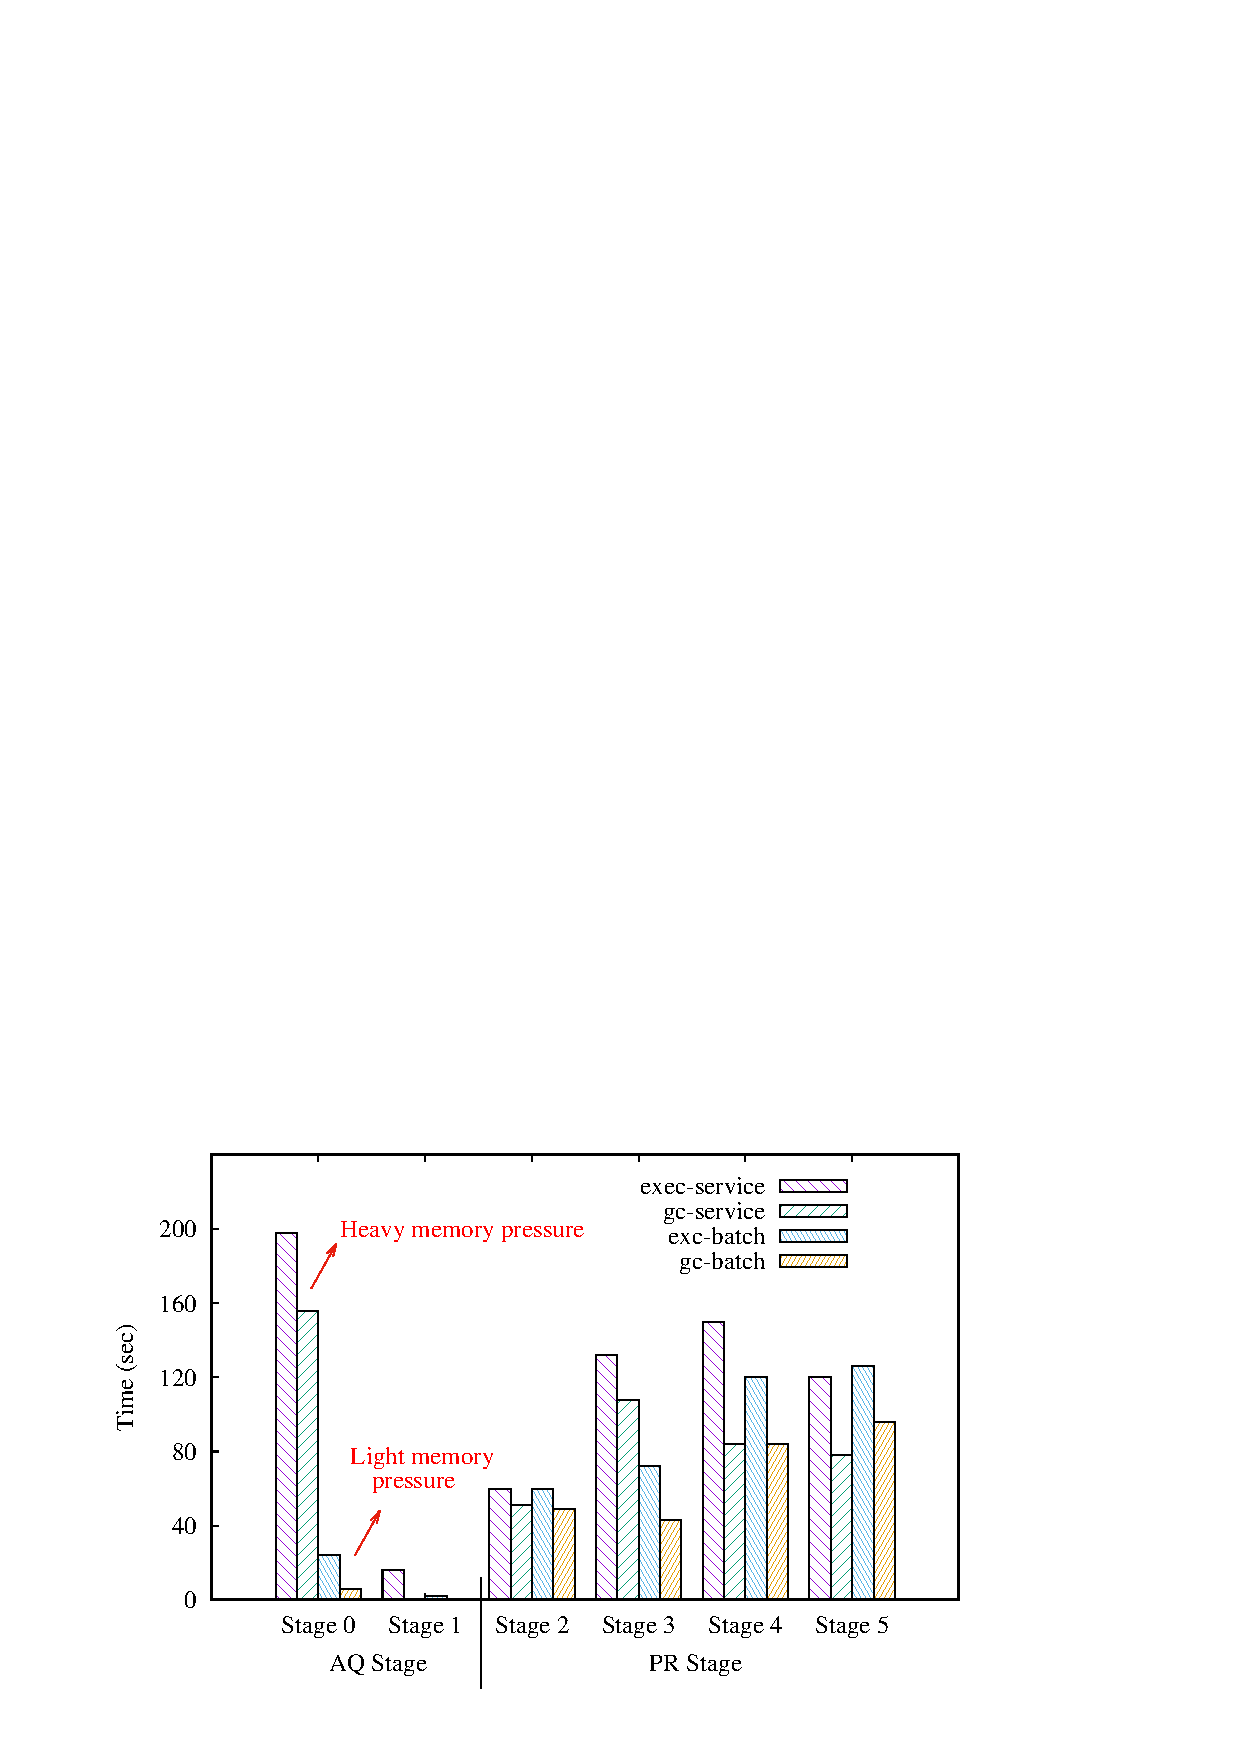
\includegraphics[width=0.35\textwidth]{motivation-exec-gc.pdf}
\vspace{-2mm}
\caption{WC suffers memory pressure from PR}
\vspace{-6mm}
\label{fig:memorypressure}
\end{figure}

\begin{comment}
\begin{figure}[!t]
\centering
\subfigure[Execution Time]{
\label{fig:subfig:mot-exec}
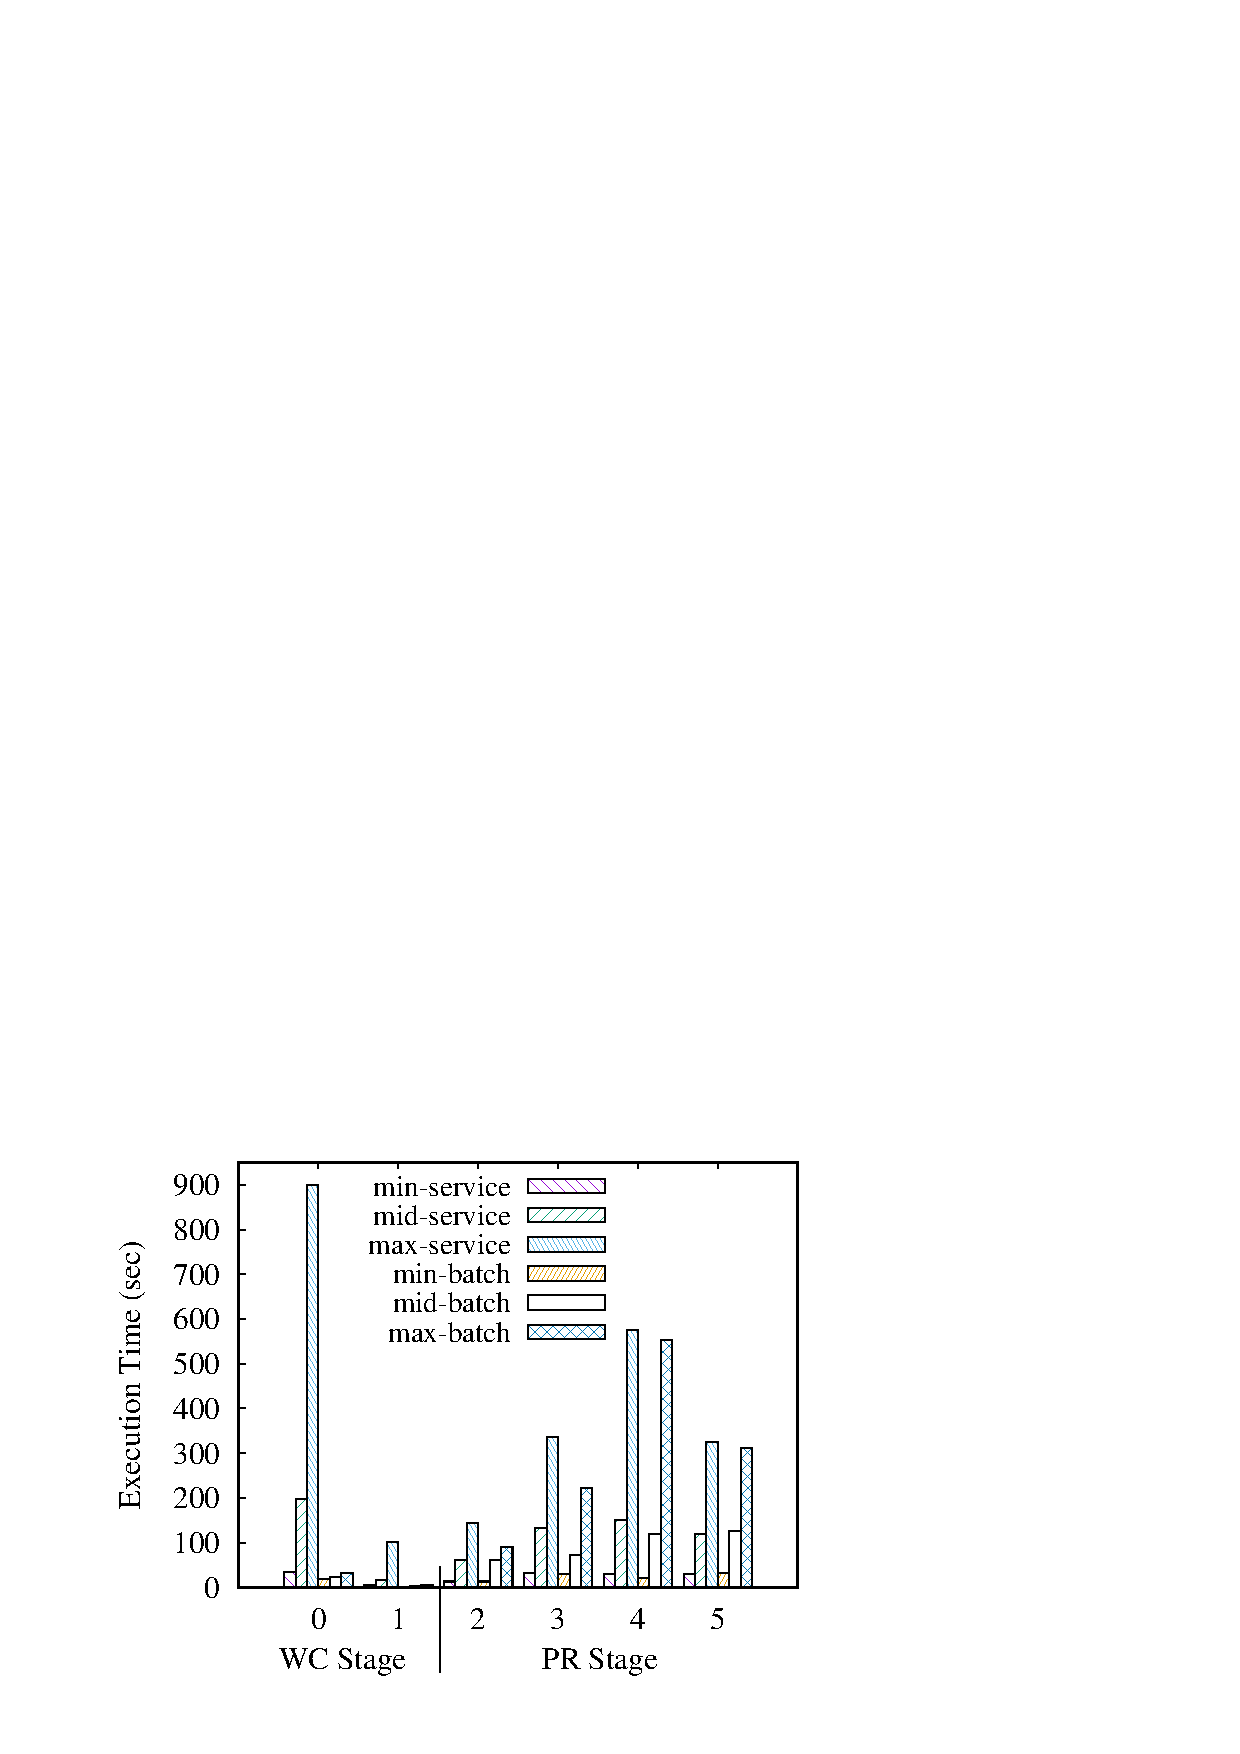
\includegraphics[width=0.231\textwidth]{motivation-exec.pdf}}
\hspace{-1.3ex}
\subfigure[GC Time]{
\label{fig:subfig:mot-gc}
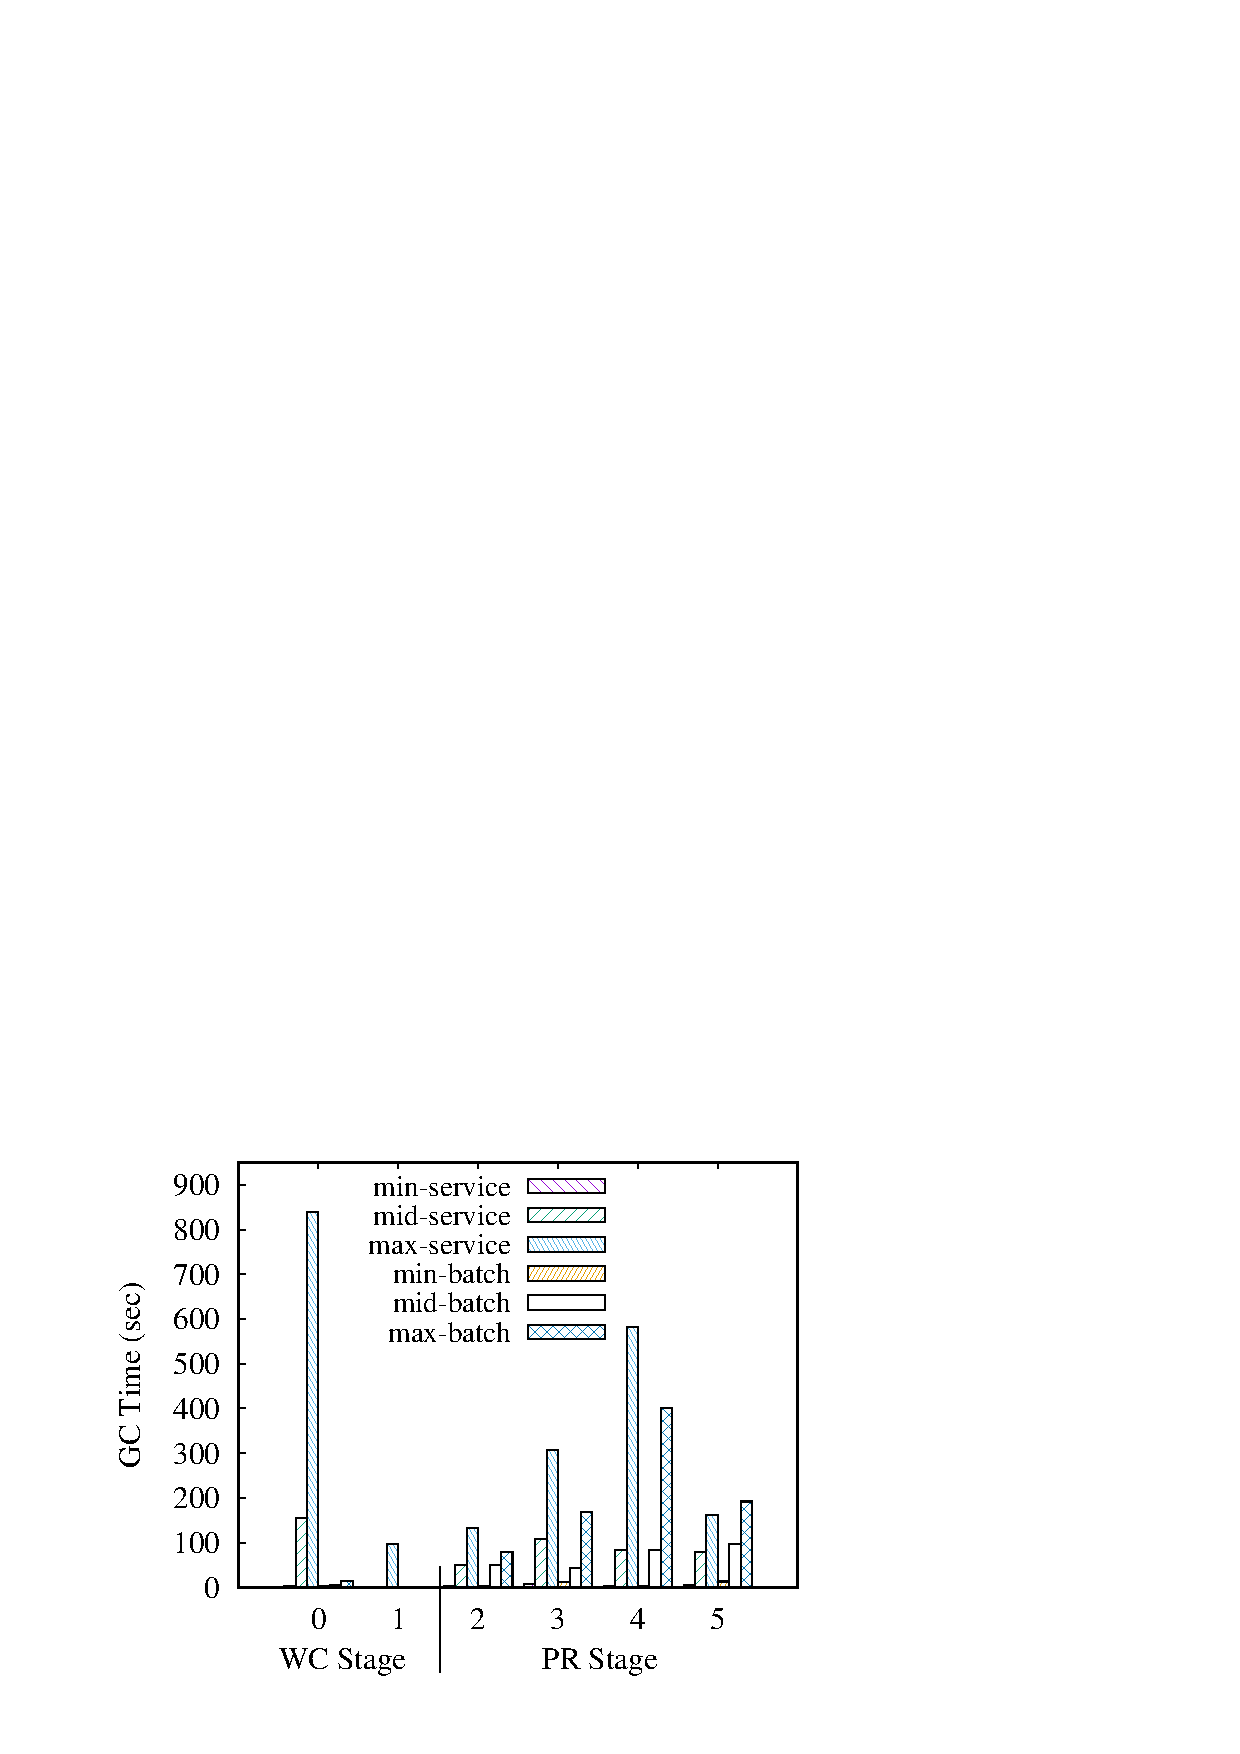
\includegraphics[width=0.231\textwidth]{motivation-gc.pdf}}
\label{fig:wc-result}
\vspace{-2mm}
\caption{The Impact of Memory Pressure}
\vspace{-2mm}
\end{figure}
\end{comment}

%Some applications, such as PR in our observation, they cache intermediate data in memory and iteratively computes the result; one iteration means a stage in Spark. Because the caching data is alive as long as the job, memory space becomes not enough for computation, which means the memory pressure is heavy in PR. However, compare with the PR, WC is another type of task, in which contains only some simple operations, just two stages and very small intermediate shuffle data--though the input data is larger than PR. Furthermore, both the execution time and garbage collection time are low in WC, and the memory pressure is much lighter than PR. The result of PR in batch processing verifies memory pressure and heavy garbage collection (exec-batch and gc-batch in Figure~\ref{fig:memorypressure}). As we can see, the garbage collection time in task accounts for a very great proportion of the execution time.

We observe that PR caches intermediate data in memory and iteratively compute the result. One iteration corresponds to one stage in Spark. Because the caching data is alive as long as the job itself, the memory space becomes gradually less and the task computation will suffer. 
%If this occurs, it indicates the memory pressure caused by PR is heavy. 
Compare with PR, however, WC only contains some simple operations. WC has only two processing stages and during its execution, a very small amount of intermediate shuffle data are generated (although the input data of WC is larger than that of PR). 
%Furthermore, both the execution time and garbage collection time are low in WC, and the memory pressure is much lighter than PR. The result of PR in the batch mode also verifies its high memory pressure and heavy garbage collection which are the results labelled as exec-batch and gc-batch in Figure~\ref{fig:memorypressure}. As we can see, the garbage collection time accounts for a very large proportion of the execution time.

%PR caches some intermediate data in memory and iteratively computes the result, each iteration means a stage in Spark. The caching data is lived as long as the job, thus available memory space for computation is less which means the memory pressure in PR is heavy. The result of PR in batch processing proves the memory pressure and heavy garbage collection (exec-batch and gc-batch in Figure~\ref{fig:memorypressure}). The garbage collection time in one task has a heavy part in the execution time. However, WC just contains some simple operations and two stages, and the intermediate shuffle data is small although the input data is larger than PR. The memory pressure in WC is light, both the execution time and the garbage collection time is low.

When multiple jobs, such as PR and WC, are submitted to and run by the Spark 
service simultaneously, the jobs are run with a fair scheduler provided by Spark. 
%Although WC has much more light memory pressure than PR, all running tasks  
%suffer from the heavy memory pressure produced by PR. 
We find that the execution time 
(exec-service in Figure~\ref{fig:memorypressure} of every task in each stage of PR has little change.
%, except some maximum execution times.
%This is because almost all memory pressure comes from PR and therefore the executions of PR in the service mode and the batch mode show similar trends. 
However, the execution of WC in the service mode is very different from that in the batch mode. This is because in the service mode, both applications are run simultaneously and therefore WC suffers from the memory pressure produced by PR even if WC is a
light task itself. 
%In the batch mode, since the applications are run one after another. The high memory pressure created by PR will not affect the running of WC.

%If PR and WC are submitted to Spark service, the submitted jobs will run with fair scheduler (provided by Spark). Although PR suffer memory pressure and WC has light memory pressure, all running tasks must suffer the heavy memory pressure produced by PR. We find that the execution time (exec-service in Figure~\ref{fig:memorypressure}) of each task in each stage has a little change in PR except some maximum values. The reason is that almost all memory pressure is coming form PR, running in Spark for service and batch processing is similar. However, WC must suffer the memory pressure produced by PR. The execution time of WC in the first stage has large fluctuation compared to that in batch processing. And we find that the extended time is almost all come from the memory pressure.

In summary, our results implicate that in a system of the service mode, 1) the heavy memory pressure will result in frequent garbage collection, which consumes most of the time and reduce the throughput; 2) the light tasks suffer from heavy memory pressure produced by the heavy tasks; and 3) the heavy tasks obtain the resources later because these resources are occupied chronically by light tasks. %and the heavy tasks themselves are the source of memory pressure.

By observing the first stage of PR and WC, we discover that the tasks of PR and WC invoke different function APIs, which determine the impact of each task on memory pressure. If we can identify and classify these tasks by the characteristics of the function APIs, we can suspend the heavy tasks and leave adequate memory space to the light tasks when the memory pressure show up. This can improve the throughput of the service-mode systems and allow all tasks to run with enough memory space and hence light memory pressure.

%Focus on the first stage of PR and WC, we discover that running tasks in PR and WC execute different function APIs. This determines the impact of each task on memory pressure. If we can identify and classify these tasks by the characteristics of function APIs implemented, while the memory pressure comes, we can suspend the heavy tasks and leave enough memory space for the light tasks. This will ensure the throughput of the system for service, and allow all tasks to run with enough memory space and without heavy memory pressure. 

%From the evaluation, we can find that when system is for service, 1) the heavy memory pressure will result in frequent garbage collection which consume most time to cut the throughput. 2) tasks with light memory pressure must suffer the heavy memory pressure produced by others. 3) tasks with heavy memory pressure will get resources later because these resources are occupied longer by these tasks with light memory pressure, and the source of memory pressure is themselves. If we can classify these tasks, when the memory pressure comes, we can stop these tasks which result in heavy memory pressure and remain enough memory space for these tasks which result in light memory pressure. It will ensure the throughput of system for service, and all tasks can run with enough memory space and without heavy memory pressure.  

%While 33\% space are cached data objects that occupy the space with long lifetime, garbage collection will not reclaim these space. We get the cost time and reclaimed space of garbage collection in Figure~\ref{fig:memorypressure}. First, the garbage collections are very frequent and the throughput of job is only 35.7\%. This proves that memory pressure is heavy in the system. Second, the cost of each garbage collection is expensive (GC Time is high in the figure). Some garbage collections which are called full GC will stop the world to mark and clean all the heap. Full GC occurs frequently because the number of lived data objects in memory is too large, it cost more time to mark the lived data objects. Too much lived data objects means less space reclaimed in each garbage collection. Thus, when less space is reclaimed (Reclaimed Space is low in the figure), more time will the garbage collection cost. The worst case is that, frequent garbage collections and less reclaimed space will hinder the performance into the vicious circle.

%Multi-tenant service is provided with the same configurations, we use WordCount, another benchmark in Spark, to balance the execution of PageRank. The dataset of WordCount is produced by HiBench~\cite{www:hibench} and the size is 50GB. The memory usage and garbage collection are the same as the batch processing. %We then consider the completion time with fair scheduler as shown in Figure~\ref{fig:memorypressure2}.
%WC has no cached data, thus memory pressure in WC is lighter and the execution time of WC can be less. However, at first, executors will be lost when jobs are submitted without any configurations tuning. The heavy memory pressure influences the output of disk and network which result in the loss of heartbeat of executors. Second, after the tuning of shuffle configurations, the throughput of WC decreases to 20\%. These tasks without producing much memory pressure must suffer the serious memory pressure from other tenants. %On the other side, PR can also benefit from WC because there are less memory pressure compared to processing batch.

\begin{comment}
\begin{figure}[!t]
\centering
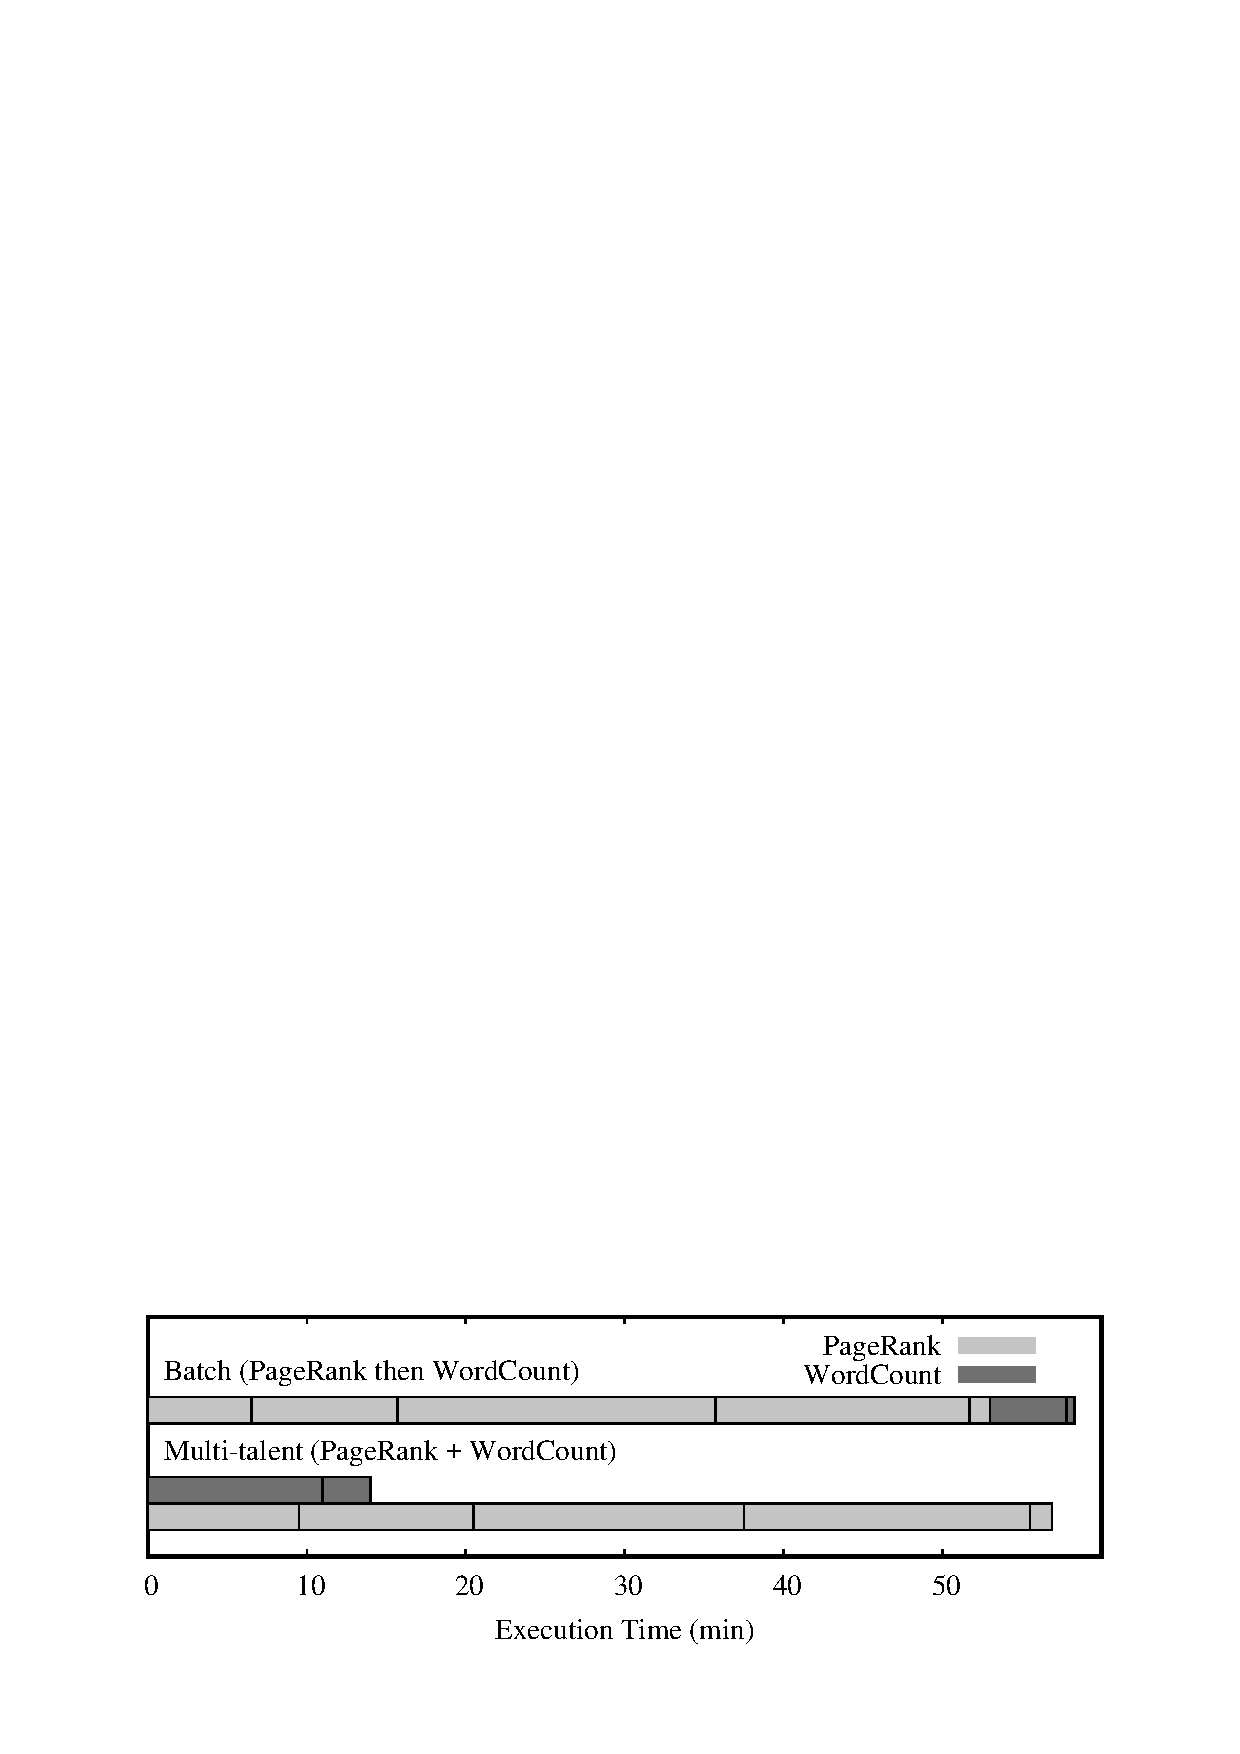
\includegraphics[width=0.45\textwidth]{memorypressure2.pdf}
\caption{Processing Batch and Mutli-tenant}
\label{fig:memorypressure2}
\end{figure}
\end{comment}

%No matter in batch processing or multi-tenant, different tasks can result in different memory pressure. Heavy memory pressure will lengthen the execution time of most tasks and decrease the throughout of jobs. The impact of memory pressure are more complex in multi-tenant in particular. Tasks with heavy memory pressure may benefit from these tasks with light memory pressure. But these tasks with light memory pressure must tolerate the memory pressure from other tasks.

%Although the framework provides several function APIs, these APIs both process the input data as key-value pairs: (key, value). All APIs process key-value pairs according to the key and user-defined functions. Some function APIs like \textit{map} just change the value; some function APIs like \textit{groupByKey} regroup values which have the same key; another function APIs like \textit{reduceByKey} aggregate values by the key. Thus, the result size of value is much different in different function APIs. For example, when one two-tuples is processed, existed key can result in the increase of value in \textit{groupByKey} but non variation in \textit{reduceByKey}. What's more, although different task implements the same function API, the result size in memory may be different because of the processing data type. Through the features of function APIs, we can classify the memory usage rate of function APIs to four type: \textbf{Constant}, \textbf{Sub-linear}, \textbf{Linear} and \textbf{Super-Linear}. After coarse-grained dividing the tasks implement function APIs to different types, when the memory pressure comes, these tasks lead to more memory pressure is clear.  
